$y=x^3$, $y=0$, $x=-1$, $x=3$

\nopagebreak
\begin{align*}
\text{El área se divide en dos partes: } & [-1,0] \text{ donde } x^3 \le 0 \\
& \text{ y } [0,3] \text{ donde } x^3 \ge 0. \\
A &= \int_{-1}^{0} (0 - x^3) \, dx + \int_{0}^{3} (x^3 - 0) \, dx \\
&= \left[ -\frac{x^4}{4} \right]_{-1}^{0} + \left[ \frac{x^4}{4} \right]_{0}^{3} \\
&= (0 - (-1/4)) + (81/4 - 0) \\
&= \frac{1}{4} + \frac{81}{4} = \frac{82}{4} = \frac{41}{2} = 20.5
\end{align*}

\[
\boxed{\displaystyle 20.5}
\]

\begin{center}
    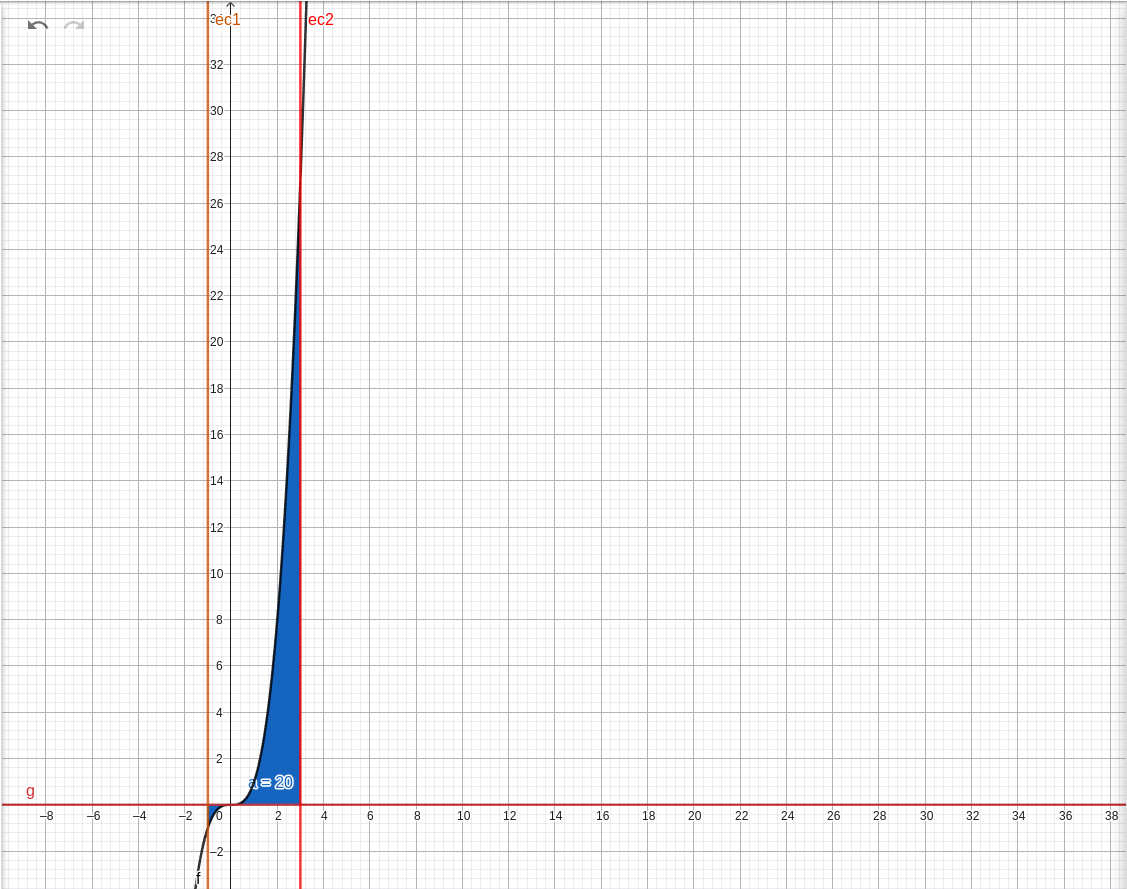
\includegraphics[width=0.5\textwidth]{Graficas/ejer16.png}
\end{center}
